\documentclass{beamer}

\title{Quantum Computing}
\subtitle{An introduction}
\author{Mitch Croal}
\date{\today}
\usetheme{Warsaw}

\usepackage{hyperref}
\usepackage{graphicx}

\newcommand{\ket}[1]{\left|{#1}\right\rangle}
\newcommand{\bra}[1]{\left\langle{#1}\right|}
\newcommand{\braket}[2]{\left\langle{#1}|{#2}\right\rangle}
\newcommand{\aop}{\textbf{A}}
\newcommand{\bop}{\textbf{B}}
\newcommand{\cop}{\textbf{C}}
\newcommand{\hop}{\textbf{H}}
\newcommand{\iop}{\textbf{1}}
\newcommand{\sop}{\textbf{S}}
\newcommand{\xop}{\textbf{X}}
\newcommand{\zop}{\textbf{Z}}
\newcommand{\zvec}{\ket{0}}
\newcommand{\ovec}{\ket{1}}
\newcommand{\xvec}[1]{\ket{x_{#1}}}

\begin{document}
  \begin{frame}
    \titlepage{}
    You can find these slides online at \url{http://z.umn.edu/acm2016quantum}
  \end{frame}

  \frame{\frametitle{Overview}\tableofcontents}

  \section{Motivation}
  \begin{frame}
    \frametitle{Motivation}
    \begin{itemize}
      \item{You can compute some things much, much faster on quantum computers}
      \begin{itemize}
        \item{Shor's algorithm can factor large numbers in polynomial time in size of the number,
          $O(\log{n}^{3})$}
        \item{Grover's Algorithm can do unstructured search in $O(\sqrt{n})$}
        \item{Quantum simulation is exponentially faster, important for physicists and chemists}
        \item{There's really a big list, can find out more here: \url{http://www.nature.com/articles/npjqi201523}}
      \end{itemize}
      \item{There's much work to be done, but there's been much progress in recent years}
      \item{D-Wave is a company that can do quantum computing right now}
    \end{itemize}
  \end{frame}

  % {{{ Introducing CBits
  \section{First steps, CBits, a classical approximation}
  \begin{frame}
    \frametitle{Units of data}
    \begin{itemize}
      \item{Binary systems with 2 states}
      \begin{itemize}
        \item{The classical bit is an example}
      \end{itemize}

      \item{Parallel to quantum information}
      \begin{itemize}
        \item{We'll first develop CBits, an analagous linear system}
        \item{From there we'll generalize to the real unit, the QBit}
      \end{itemize}
    \end{itemize}
  \end{frame}

  \begin{frame}
    \frametitle{Introducing CBits}
    \begin{itemize}
      \item{A single CBit}
        \begin{itemize}
          \item{The `state space' is a two-dimensional vector space}
          \item{Spanned by 2 orthonormal vectors, $\zvec$ and $\ovec$} 
          $\zvec = \begin{pmatrix}1\\0\end{pmatrix},
           \ovec = \begin{pmatrix}0\\1\end{pmatrix}$
        \end{itemize}
    \end{itemize}
    \begin{itemize}
      \item{Systems of multiple CBits}
        \begin{itemize}
          \item{We need a way to mathematically combine CBits}
          \item{Can do so with the so-called `tensor product', denoted by $\otimes$} 
        \end{itemize}
    \end{itemize}
  \end{frame}

  \begin{frame}
    \frametitle{Tensor Products}

    The tensor product of column vectors looks like this: \\

    $\begin{pmatrix}a_{1}\\a_{2}\end{pmatrix} \otimes \begin{pmatrix}b_{1}\\b_{2}\end{pmatrix} = 
     \begin{pmatrix}a_{1}\begin{pmatrix}b_{1}\\b_{2}\end{pmatrix} \\ 
        a_{2}\begin{pmatrix}b_{1}\\b_{2}\end{pmatrix}\end{pmatrix} = 
     \begin{pmatrix}a_{1}b_{1}\\a_{1}b_{2}\\a_{2}b_{1}\\a_{2}b_{2}\end{pmatrix} $
  \end{frame}

  \begin{frame}
    \frametitle{Multiple CBits}
    \begin{itemize}
      \item{State space of multiple CBits}
        \begin{itemize}
          \item{Basis vectors are pairwise tensor products of $\zvec$ and $\ovec$}
          \item{$\zvec \otimes \zvec$, $\zvec \otimes \ovec$ $\ovec \otimes \zvec$, $\ovec \otimes \ovec$}
          \item{We now have a 4-dimensional vector space}
        \end{itemize}
    \end{itemize}

    $\zvec \otimes \zvec = \begin{pmatrix}1\\0\\0\\0\end{pmatrix}, 
     \zvec \otimes \ovec = \begin{pmatrix}0\\1\\0\\0\end{pmatrix}, \linebreak
     \ovec \otimes \zvec = \begin{pmatrix}0\\0\\1\\0\end{pmatrix},
     \ovec \otimes \ovec = \begin{pmatrix}0\\0\\0\\1\end{pmatrix}$
  \end{frame}
  
  \begin{frame}
    \frametitle{Multiple CBits Notation}
    \begin{itemize}
      \item{Often we can leave out the $\otimes$} \linebreak
      $\zvec\zvec \quad \zvec\ovec \quad \ovec\zvec \quad \ovec\ovec$
      \item{For even more readability} \linebreak
      $\ket{00} \quad \ket{01} \quad \ket{10} \quad \ket{11}$
      \item{We can write them in decimal instead, with a subscore to indicate number of CBits} \linebreak
      $\ket{0}_{2} \quad \ket{1}_{2} \quad \ket{2}_{2} \quad \ket{3}_{2}$
      \item{We can then generalize this to systems of $n$ Cbits, with the following basis vectors} \linebreak
      $\ket{x}_{n}$, $0 \leq x < 2^{n}$
    \end{itemize}
  \end{frame}
  % }}}

  % {{{ Operations on CBits
  \section{Operations on CBits}
  \subsection{Properties of Quantum Information}
  \begin{frame} 
    \frametitle{CBits and QBits}
    \begin{itemize}
      \item{CBits are closely related to the `real' unit of quantum information, the QBit}
      \begin{itemize}
        \item{Usually written as \textit{qubit}}
      \end{itemize}
      \item{QBits are realized by actual physical two-state systems}
      \begin{itemize}
        \item{Operations on the states of QBits must be reversible}
        \item{With a single exception, `measurement', which we'll discuss later}
        \item{We'll therefore only consider reversible operations on CBits}
      \end{itemize}
    \end{itemize}
  \end{frame}
  % }}}

  % {{{ Single CBit case
  \subsection{Single CBit case}
  \begin{frame}
    \frametitle{Single CBit operations}
    \begin{itemize}
      \item{Reversibility constrains us a bit}
      \begin{itemize}
        \item{Operations like \textit{erase}, $\zvec \rightarrow \zvec, \ovec \rightarrow \zvec$, are disallowed}
      \end{itemize}
      \item{Therefore only 2 meaningful operations on CBits}
      \begin{itemize}
        \item{The identity operator, $\iop$} \linebreak
        $\iop\zvec = \zvec, \iop\ovec = \ovec$
        \item{The swap operator, $\xop$} \linebreak
        $\xop\zvec = \ovec, \xop\ovec = \zvec$
      \end{itemize}
      \item{However, `meaningless' operations can be made useful}
      \begin{itemize}
        \item{Introduce the $\zop$ operator} \linebreak
        $\zop\zvec = \zvec, \zop\ovec = -\ovec$
      \end{itemize}
      \item{What the heck is $-\ovec$?}
    \end{itemize}
  \end{frame}
  % }}}

  % {{{ Multiple CBit operations
  \subsection{Multiple CBits}
  \begin{frame}
    \frametitle{Multiple CBit operations}
    \begin{itemize}
      \item{It's useful to have compact notation for operators that act on many qubits}
      \begin{itemize}
        \item{Begin by labelling each qubit $0,1,2,\ldots$} \linebreak
        \item{Thus if $x$ has the binary expansion $x=8x_{3}+4x_{2}+2x_{1}+x_{0}$}
        \begin{align*}
        \ket{x}_{4} = \ket{x_{3}x_{2}x_{1}x_{0}} &= \ket{x_{3}} \ket{x_{2}} \ket{x_{1}} \ket{x_{0}} \\
                    &= \ket{x_{3}} \otimes \ket{x_{2}} \otimes \ket{x_{1}} \otimes \ket{x_{0}}
        \end{align*}
      \end{itemize}

      \item{An operation that acts only on Cbit \#2 is} \linebreak
      $\xop_{2}=\iop \otimes \xop \otimes \iop \otimes \iop$
      \item{It follows from the definition of our tensor product that} \linebreak
      $\xop [ \ \ket{x_{3}} \otimes  \ket{x_{2}} \otimes \ket{x_{1}}\otimes  \ket{x_{0}} \ ] = 
       \ket{x_{3}} \otimes [ \ \xop \ket{x_{2}} \ ] \otimes \ket{x_{1}} \otimes \ket{x_{0}} $
    \end{itemize}
  \end{frame}

  \begin{frame}
    \frametitle{Multiple CBit operations}
    \begin{itemize}
      \item{Less trivial operations are available when working with multiple CBits}
      \begin{itemize}
        \item{The swap operator, $\sop$} \linebreak
          $\sop\ket{xy} = \ket{yx}$
        \item{The controlled `not', $\cop$} \linebreak
          $\cop\ket{0x} = \zvec\ket{x}, \cop\ovec\ket{x} = \ovec\ket{\neg x}$
      \end{itemize}
      \item{We can build up these operations using `meaningless' operators, like $\zop$}
      \item{First consider the operator $\aop = \frac{1}{2}(\iop + \zop_{1}\zop_{0})$}
      \begin{itemize}
        \item{$\aop$ acts as the identity on the 2 states $\ket{00}$ and $\ket{11}$}
        \item{$\aop$ gives $0$ (clasically meaningless) for $\ket{01}$ and $\ket{10}$}
      \end{itemize}
    \end{itemize}
  \end{frame}

  \begin{frame}
    \frametitle{Multiple CBit operations}
    \begin{itemize}
      \item{The \textit{Hadamard} operator, $\hop$, is particularly well known} \linebreak
        $\hop = \frac{1}{\sqrt{2}}(\xop + \zop) =
         \frac{1}{\sqrt{2}} \begin{pmatrix}1 & 1 \\ 1 & -1\end{pmatrix}$
         \item{$\hop$, like $\zop$, can be used to build up useful multi-CBit operations}
    \end{itemize}
  \end{frame}
  % }}}

  % {{{ Quantum Bits, QBits
  \section{Quantum Bits, QBits}
  \subsection{Properties of QBits}
  \begin{frame}
    \frametitle{QBits}
    \begin{itemize}
      \item{QBits, the units of quantum information, are much like CBits}
      \begin{itemize}
        \item{General form of the CBit is $a\zvec + b\ovec$}
        \item{General form of the QBit is $\alpha\zvec + \beta\ovec$}, where $\alpha$
          and $\beta$ are complex numbers
      \end{itemize}
    \item{Quantum states are also subject to the \textit{normalization} condition}
      \begin{itemize}
        \item{$|\alpha|^{2} + |\beta|^{2} = 1$}
      \end{itemize}
      \item{This is because QBits correspond to actual `observables'}
      \begin{itemize}
        \item{The probability of observing state $\ket{x}_{n}$ corresponds to its `probability amplitude'}
        \item{Coin demonstration, $\frac{1}{\sqrt{2}}(\zvec + \ovec)$}
      \end{itemize}
      \item{Generalizing to $n$ QBits, the general form is this:} \linebreak
        $\ket{\psi} =  \sum\limits_{0 \leq x < 2^{n}}a_{x}\ket{x}$
    \end{itemize}
  \end{frame}

  \subsection{Quantum properties}
  \begin{frame}
    \frametitle{Quantum Wierdness}
    \begin{itemize}
      \item{Quantum computing deals heavily with \textit{hidden information}}
      \begin{itemize}
        \item{We're often given a state $\ket{\psi}$, but we don't know the coefficients, which can be arbitrarily precise}
        \item{A set of $n$ QBits has $2^{n}$ amplitudes corresponding to each combination of $\zvec$ and $\ovec$}
        \item{Operators like $\zop$ and $\hop$ can be chained to operate on all this data at once!}
      \end{itemize}
      \item{Pretty cool, right? There's a catch}
      \item{Measurement collapses quantum states}
      \begin{itemize}
        \item{Remember the coin?}
        \item{We didn't know before, but after we knew, it didn't change}
      \end{itemize}
    \end{itemize}
  \end{frame}
  % }}}

  % {{{ Quantum Algorithms
  \subsection{Quantum Algorithms}
  \begin{frame}
    \frametitle{Quantum Algorithms}
    \begin{itemize}
      \item{Doing real work with quantum circuits are notoriously tricky}
      \begin{itemize}
        \item{How do you even get any useful information when it's all random?}
        \item{At a high level, it's all about reinforcing the amplitudes you want,
          diminishing the rest, and then measuring}
      \end{itemize}
      \item{I think a real example of how this all comes together would be helpful}
    \end{itemize}
  \end{frame}
  % }}}

  \subsection{Quantum Circuits}
  \begin{frame}
    \frametitle{Anatomy of a Quantum Circuit}
    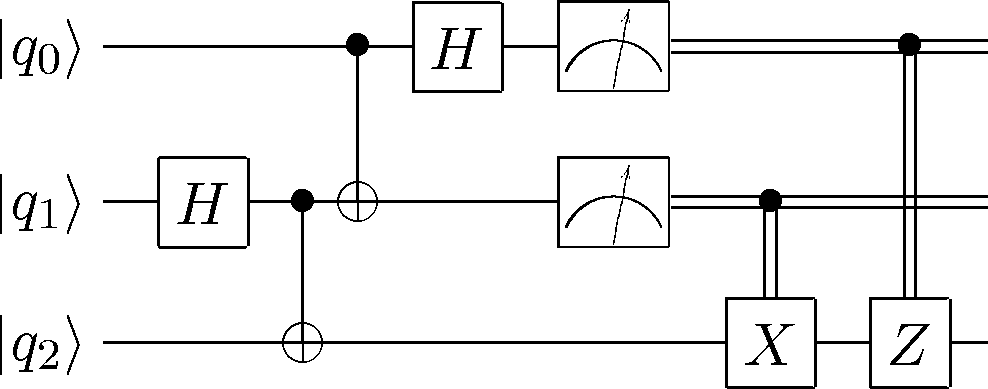
\includegraphics[height=100px,width=300px]{circuit.png}
    \begin{itemize}
      \item{Inputs on the left, each line corresponds to a single QBit}
      \item{The boxes are operators (or gates)}
      \begin{itemize}
        \item{$\hop$ is the Hadamard Gate, $\xop$ and $\zop$ are the Pauli X and Z}
      \end{itemize}
      \item{The meters do measurement, and collapse the measured QBit}
      \item{The black dots and lines indicate control QBits}
    \end{itemize}
  \end{frame}
\end{document}
